% Options for packages loaded elsewhere
\PassOptionsToPackage{unicode}{hyperref}
\PassOptionsToPackage{hyphens}{url}
%
\documentclass[
]{book}
\usepackage{amsmath,amssymb}
\usepackage{lmodern}
\usepackage{iftex}
\ifPDFTeX
  \usepackage[T1]{fontenc}
  \usepackage[utf8]{inputenc}
  \usepackage{textcomp} % provide euro and other symbols
\else % if luatex or xetex
  \usepackage{unicode-math}
  \defaultfontfeatures{Scale=MatchLowercase}
  \defaultfontfeatures[\rmfamily]{Ligatures=TeX,Scale=1}
\fi
% Use upquote if available, for straight quotes in verbatim environments
\IfFileExists{upquote.sty}{\usepackage{upquote}}{}
\IfFileExists{microtype.sty}{% use microtype if available
  \usepackage[]{microtype}
  \UseMicrotypeSet[protrusion]{basicmath} % disable protrusion for tt fonts
}{}
\makeatletter
\@ifundefined{KOMAClassName}{% if non-KOMA class
  \IfFileExists{parskip.sty}{%
    \usepackage{parskip}
  }{% else
    \setlength{\parindent}{0pt}
    \setlength{\parskip}{6pt plus 2pt minus 1pt}}
}{% if KOMA class
  \KOMAoptions{parskip=half}}
\makeatother
\usepackage{xcolor}
\usepackage{color}
\usepackage{fancyvrb}
\newcommand{\VerbBar}{|}
\newcommand{\VERB}{\Verb[commandchars=\\\{\}]}
\DefineVerbatimEnvironment{Highlighting}{Verbatim}{commandchars=\\\{\}}
% Add ',fontsize=\small' for more characters per line
\usepackage{framed}
\definecolor{shadecolor}{RGB}{248,248,248}
\newenvironment{Shaded}{\begin{snugshade}}{\end{snugshade}}
\newcommand{\AlertTok}[1]{\textcolor[rgb]{0.94,0.16,0.16}{#1}}
\newcommand{\AnnotationTok}[1]{\textcolor[rgb]{0.56,0.35,0.01}{\textbf{\textit{#1}}}}
\newcommand{\AttributeTok}[1]{\textcolor[rgb]{0.77,0.63,0.00}{#1}}
\newcommand{\BaseNTok}[1]{\textcolor[rgb]{0.00,0.00,0.81}{#1}}
\newcommand{\BuiltInTok}[1]{#1}
\newcommand{\CharTok}[1]{\textcolor[rgb]{0.31,0.60,0.02}{#1}}
\newcommand{\CommentTok}[1]{\textcolor[rgb]{0.56,0.35,0.01}{\textit{#1}}}
\newcommand{\CommentVarTok}[1]{\textcolor[rgb]{0.56,0.35,0.01}{\textbf{\textit{#1}}}}
\newcommand{\ConstantTok}[1]{\textcolor[rgb]{0.00,0.00,0.00}{#1}}
\newcommand{\ControlFlowTok}[1]{\textcolor[rgb]{0.13,0.29,0.53}{\textbf{#1}}}
\newcommand{\DataTypeTok}[1]{\textcolor[rgb]{0.13,0.29,0.53}{#1}}
\newcommand{\DecValTok}[1]{\textcolor[rgb]{0.00,0.00,0.81}{#1}}
\newcommand{\DocumentationTok}[1]{\textcolor[rgb]{0.56,0.35,0.01}{\textbf{\textit{#1}}}}
\newcommand{\ErrorTok}[1]{\textcolor[rgb]{0.64,0.00,0.00}{\textbf{#1}}}
\newcommand{\ExtensionTok}[1]{#1}
\newcommand{\FloatTok}[1]{\textcolor[rgb]{0.00,0.00,0.81}{#1}}
\newcommand{\FunctionTok}[1]{\textcolor[rgb]{0.00,0.00,0.00}{#1}}
\newcommand{\ImportTok}[1]{#1}
\newcommand{\InformationTok}[1]{\textcolor[rgb]{0.56,0.35,0.01}{\textbf{\textit{#1}}}}
\newcommand{\KeywordTok}[1]{\textcolor[rgb]{0.13,0.29,0.53}{\textbf{#1}}}
\newcommand{\NormalTok}[1]{#1}
\newcommand{\OperatorTok}[1]{\textcolor[rgb]{0.81,0.36,0.00}{\textbf{#1}}}
\newcommand{\OtherTok}[1]{\textcolor[rgb]{0.56,0.35,0.01}{#1}}
\newcommand{\PreprocessorTok}[1]{\textcolor[rgb]{0.56,0.35,0.01}{\textit{#1}}}
\newcommand{\RegionMarkerTok}[1]{#1}
\newcommand{\SpecialCharTok}[1]{\textcolor[rgb]{0.00,0.00,0.00}{#1}}
\newcommand{\SpecialStringTok}[1]{\textcolor[rgb]{0.31,0.60,0.02}{#1}}
\newcommand{\StringTok}[1]{\textcolor[rgb]{0.31,0.60,0.02}{#1}}
\newcommand{\VariableTok}[1]{\textcolor[rgb]{0.00,0.00,0.00}{#1}}
\newcommand{\VerbatimStringTok}[1]{\textcolor[rgb]{0.31,0.60,0.02}{#1}}
\newcommand{\WarningTok}[1]{\textcolor[rgb]{0.56,0.35,0.01}{\textbf{\textit{#1}}}}
\usepackage{longtable,booktabs,array}
\usepackage{calc} % for calculating minipage widths
% Correct order of tables after \paragraph or \subparagraph
\usepackage{etoolbox}
\makeatletter
\patchcmd\longtable{\par}{\if@noskipsec\mbox{}\fi\par}{}{}
\makeatother
% Allow footnotes in longtable head/foot
\IfFileExists{footnotehyper.sty}{\usepackage{footnotehyper}}{\usepackage{footnote}}
\makesavenoteenv{longtable}
\usepackage{graphicx}
\makeatletter
\def\maxwidth{\ifdim\Gin@nat@width>\linewidth\linewidth\else\Gin@nat@width\fi}
\def\maxheight{\ifdim\Gin@nat@height>\textheight\textheight\else\Gin@nat@height\fi}
\makeatother
% Scale images if necessary, so that they will not overflow the page
% margins by default, and it is still possible to overwrite the defaults
% using explicit options in \includegraphics[width, height, ...]{}
\setkeys{Gin}{width=\maxwidth,height=\maxheight,keepaspectratio}
% Set default figure placement to htbp
\makeatletter
\def\fps@figure{htbp}
\makeatother
\setlength{\emergencystretch}{3em} % prevent overfull lines
\providecommand{\tightlist}{%
  \setlength{\itemsep}{0pt}\setlength{\parskip}{0pt}}
\setcounter{secnumdepth}{5}
\usepackage{booktabs}
\usepackage{amsthm}
\makeatletter
\def\thm@space@setup{%
  \thm@preskip=8pt plus 2pt minus 4pt
  \thm@postskip=\thm@preskip
}
\makeatother
\ifLuaTeX
  \usepackage{selnolig}  % disable illegal ligatures
\fi
\usepackage[]{natbib}
\bibliographystyle{apalike}
\IfFileExists{bookmark.sty}{\usepackage{bookmark}}{\usepackage{hyperref}}
\IfFileExists{xurl.sty}{\usepackage{xurl}}{} % add URL line breaks if available
\urlstyle{same} % disable monospaced font for URLs
\hypersetup{
  pdftitle={Modul Praktikum Aplikasi Komputer dengan R},
  pdfauthor={Dimas Wicaksono},
  hidelinks,
  pdfcreator={LaTeX via pandoc}}

\title{Modul Praktikum Aplikasi Komputer dengan R}
\author{Dimas Wicaksono}
\date{2023-07-16}

\begin{document}
\maketitle

{
\setcounter{tocdepth}{1}
\tableofcontents
}
\hypertarget{pendahuluan}{%
\chapter*{Pendahuluan}\label{pendahuluan}}
\addcontentsline{toc}{chapter}{Pendahuluan}

This is a \emph{sample} book written in \textbf{Markdown}. You can use anything that Pandoc's Markdown supports, e.g., a math equation \(a^2 + b^2 = c^2\). \protect\hyperlink{a1-pengenalan}{Acara 1}.

The \textbf{bookdown} package can be installed from CRAN or Github:

\begin{Shaded}
\begin{Highlighting}[]
\FunctionTok{install.packages}\NormalTok{(}\StringTok{"bookdown"}\NormalTok{)}
\CommentTok{\# or the development version}
\CommentTok{\# devtools::install\_github("rstudio/bookdown")}
\end{Highlighting}
\end{Shaded}

Remember each Rmd file contains one and only one chapter, and a chapter is defined by the first-level heading \texttt{\#}.

To compile this example to PDF, you need XeLaTeX. You are recommended to install TinyTeX (which includes XeLaTeX): \url{https://yihui.name/tinytex/}.

\hypertarget{a1-pengenalan}{%
\chapter{Pengenalan Statistik dengan R}\label{a1-pengenalan}}

\hypertarget{a2-deskriptif}{%
\chapter{Statistik Deskriptif}\label{a2-deskriptif}}

\hypertarget{prinsip}{%
\section{PRINSIP}\label{prinsip}}

Statistik Deskriptif adalah sebuah metode statistika yang bertujuan untuk mendapatkan ringkasan dari data. Ringkasan ini akan memberikan gambaran tentang distribusi dari data. Statistik deskriptif sangat penting dilakukan sebelum melakukan pengolahan data, bahkan digunakan untuk penentuan awal dalam melakukan manajemen data. Ukuran-ukuran dalam statistik deskriptif mencakup ukuran pemusatan dan penyebaran dari data. Ukuran pemusatan terdiri dari nilai rerata, median dan modus. Sedangkan ukuran penyebaran terdiri dari nilai ragam, standar deviasi, nilai minimum dan maksimum, serta nilai keruncingan (kurtosis) dan kemiringan (skewness). Perlu diketahui, bahwa ukuran pemusatan dan penyebaran ini hanya dapat dilakukan pada skala data interval dan rasio.

\hypertarget{capaian-pembelajaran-lulusan}{%
\section{CAPAIAN PEMBELAJARAN LULUSAN}\label{capaian-pembelajaran-lulusan}}

\hypertarget{capaian-pembelajaran-mata-kuliah}{%
\section{CAPAIAN PEMBELAJARAN MATA KULIAH}\label{capaian-pembelajaran-mata-kuliah}}

\hypertarget{a2-materi}{%
\section{MATERI}\label{a2-materi}}

\hypertarget{ukuran-pemusatan-data}{%
\subsection{Ukuran Pemusatan Data}\label{ukuran-pemusatan-data}}

Dalam pengolahan data, sangat penting bagi peneliti untuk mengetahui bagaimana ringkasan dari data. Adanya informasi tersebut akan menjadi dasar dalam pemilihan metode pengolahan data. Ukuran Pemusatan Data merupakan statistik dapat memberikan ringkasan pada data yang menunjukkan nilai tengah atau keterpusatan data.

\hypertarget{rerata-mean}{%
\subsubsection{Rerata (Mean)}\label{rerata-mean}}

Rerata merupakan nilai yang sering digunakan untuk mewakili data. Hal ini dikarenakan rerata cenderung memusat, berada pada tengah-tengah data. Perhatikan contoh pada Gambar berikut:

\begin{figure}

{\centering 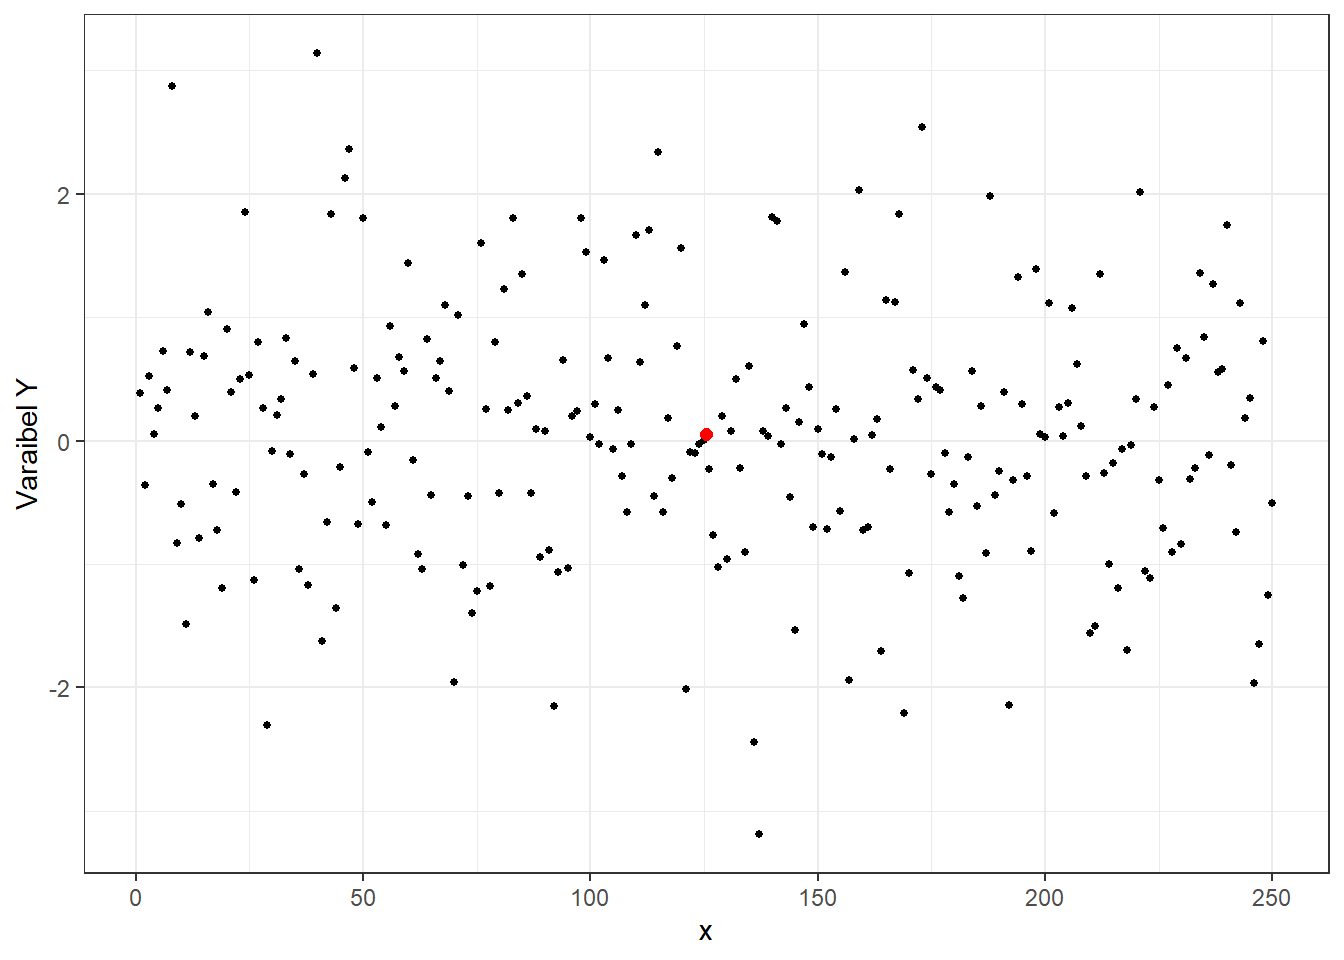
\includegraphics{Aplikasi-Komputer---Biostatistika_files/figure-latex/a2-fig1-1} 

}

\caption{Contoh Data dan Nilai Reratanya}\label{fig:a2-fig1}
\end{figure}

Perhatikan bahwa pada \protect\hyperlink{fig:a2-fig1}{Gambar 2.1} terdapat sebuah data yang diwakili dengan titik hitam dan nilai reratanya yang diwakili oleh warna merah. Titik merah yang merupakan nilai rerata berada pada tengah-tengah data, meskipun tidak harus persis berada ditengah.

Fungsi yang digunakan untuk mendapatkan nilai rerata pada Program R adalah \texttt{mean(data)}. Ubah ``data'' dengan objek data yang digunakan. Semisal saya memiliki objek data dengan nama \texttt{mydata}, maka penggunaan fungsi tersebut adalah sebagai berikut:

\begin{Shaded}
\begin{Highlighting}[]
\FunctionTok{mean}\NormalTok{(mydata)}
\end{Highlighting}
\end{Shaded}

\hypertarget{median}{%
\subsubsection{Median}\label{median}}

Berbeda dengan rerata yang posisinya tidak tepat pada tengah-tengah data, median adalah nilai yang tepat berada di tengah-tengah data. Nilai median dapat digunakan sebagai nilai yang mewakili data jika nilai rerata dianggap kurang merepresentasikan pusat data. Ini biasanya terjadi pada data dengan distribusi data yang tidak seimbang. Selain itu, nilai median juga lebih diterima pada data-data hasil perhitungan, dimana data ini tidak memiliki nilai desimal.

Untuk mendapatkan nilai median pada data, gunakan fungsi \texttt{median(data)}. Ubah ``data'' dengan objek data yang digunakan.

\begin{Shaded}
\begin{Highlighting}[]
\FunctionTok{median}\NormalTok{(mydata)}
\end{Highlighting}
\end{Shaded}

\hypertarget{a2-modus}{%
\subsubsection{Modus}\label{a2-modus}}

Nilai Modus merupakan nilai data yang paling sering muncul. Nilai modus sering digunakan untuk membandingkan nilai tersebut dengan median ataupun reratanya. Nilai modus yang lebih besar dari nilai median dan rerata menunjukkan bahwa distribusi data miring ke kiri sedangkan nilai modus yang kurang dari nilai median dan rerata menunjukkan bahwa distribusi data miring ke kanan. Perhatikan gambar berikut:

\begin{figure}

{\centering 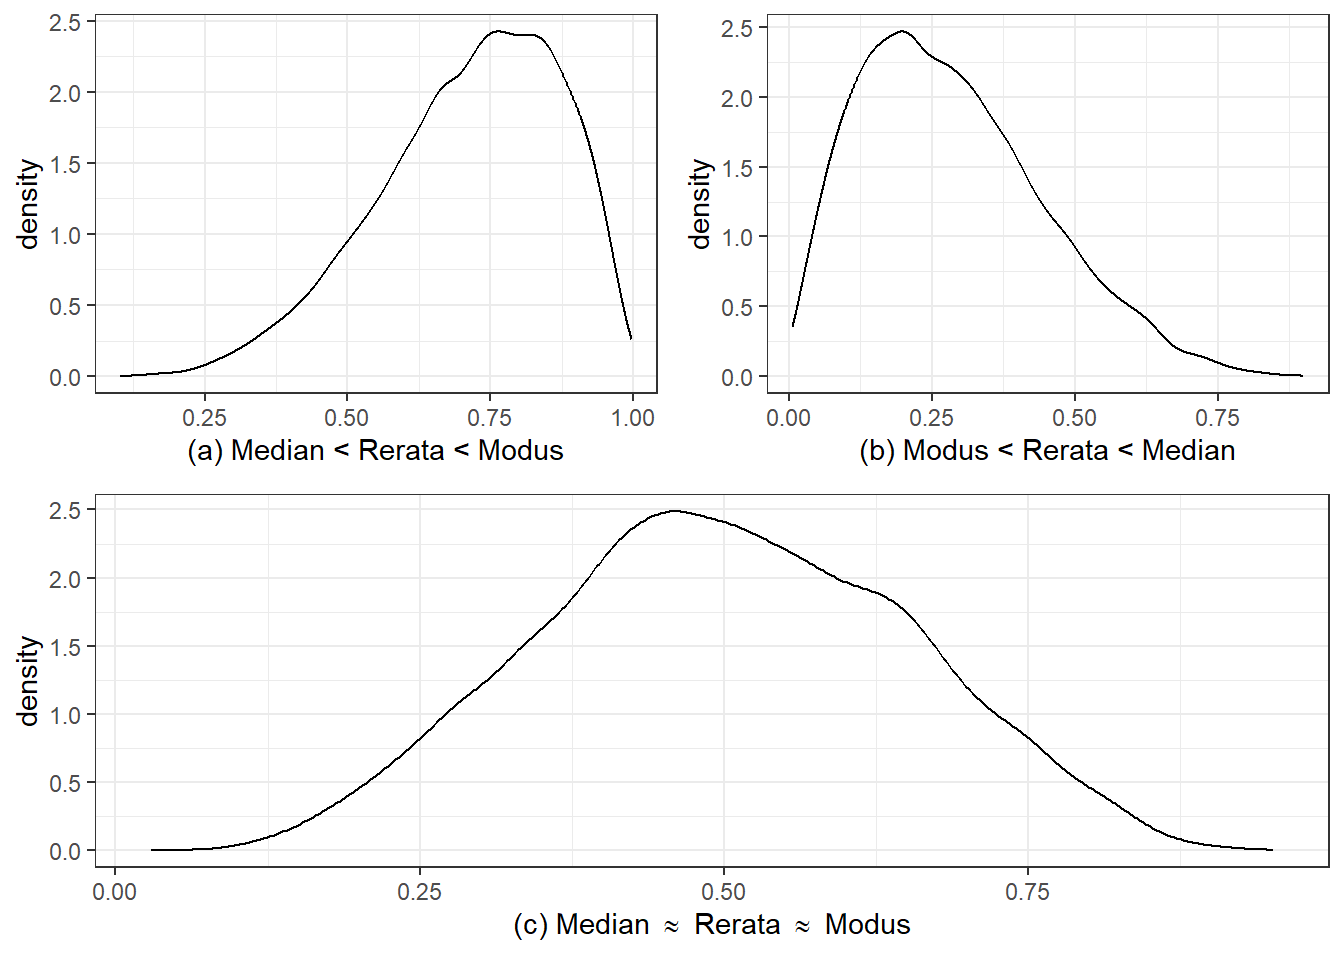
\includegraphics{Aplikasi-Komputer---Biostatistika_files/figure-latex/a2-fig2-1} 

}

\caption{Distribusi Data berdasarkan Nilai Rerata, Median dan Modusnya}\label{fig:a2-fig2}
\end{figure}

Penjelasan \href{fig:a2-fig2}{Gambar 2.2}.

Mendapatkan modus pada data di Program R tidak seperti mendapatkan rerata dan median. Fungsi modus perlu dibuat secara manual. Berikut adalah contoh fungsi modus:

\begin{Shaded}
\begin{Highlighting}[]
\NormalTok{modus }\OtherTok{=} \ControlFlowTok{function}\NormalTok{(x) \{}
\NormalTok{  nilai\_unik }\OtherTok{=} \FunctionTok{unique}\NormalTok{(x)}
\NormalTok{  tabel\_nilai\_unik }\OtherTok{=} \FunctionTok{tabulate}\NormalTok{(}\FunctionTok{match}\NormalTok{(x, nilai\_unik))}
\NormalTok{  modus\_nilai\_unik }\OtherTok{=}\NormalTok{ nilai\_unik[}\FunctionTok{which.max}\NormalTok{(tabel\_nilai\_unik)]}
  \FunctionTok{return}\NormalTok{(modus\_nilai\_unik)}
\NormalTok{\}}
\end{Highlighting}
\end{Shaded}

Selanjutnya kita dapat menggunakan fungsi tersebut untuk mendapatkan modus dengan cara:

\begin{Shaded}
\begin{Highlighting}[]
\FunctionTok{modus}\NormalTok{(mydata)}
\end{Highlighting}
\end{Shaded}

\hypertarget{ukuran-penyebaran-data}{%
\subsection{Ukuran Penyebaran Data}\label{ukuran-penyebaran-data}}

Telah dipelajari sebelumnya bahwa ukuran pemusatan dapat memberikan nilai-nilai yang direpresentasikan sebagai pusat dari data. Meski demikian, ada banyak data riil yang memiliki keragaman nilai yang sangat tinggi. Akibatnya, nilai ukuran pemusatan tidak dapat memberikan informasi yang cukup. Ukuran penyebaran memberikan ringkasan dari penyebaran data. Perhatikan data berikut:

\begin{table}

\caption{\label{tab:a2-tab1}Data Kadar HB Wanita Hamil}
\centering
\begin{tabular}[t]{c|c|c}
\hline
ID & Penambah\_Darah & HB\\
\hline
1 & Ya & 11.00\\
\hline
2 & Ya & 12.25\\
\hline
3 & Ya & 11.06\\
\hline
4 & Ya & 11.43\\
\hline
5 & Ya & 11.64\\
\hline
6 & Tidak & 6.39\\
\hline
7 & Tidak & 11.66\\
\hline
8 & Tidak & 7.82\\
\hline
9 & Tidak & 7.67\\
\hline
10 & Tidak & 7.56\\
\hline
\end{tabular}
\end{table}

Perhatikan \protect\hyperlink{tab:a2-tab1}{Tabel 2.1}, ID menunjukkan ID dari responden, kolom Penambah.Darah merupakan status kepatuhan responden dalam konsumsi tablet tambah darah, dan kolom KB adalah kadar KB responden. Pada tabel itu menunjukkan bahwa rerata kadar HB pada responden yang mengonsumsi tabel tambah darah adalah sebesar \texttt{11.5}, sedangkan rerata yang tidak adalah \texttt{8.22}. Pada data ini, kita dapat menduga bahwa responden yang tidak patuh dalam mengonsumsi penambah darah seolah-olah tidak memerlukan tindakan yang serius. Padahal salah satu responden telah memiliki kadar HB \textless{} 7.

Ringkasan data pada \protect\hyperlink{tab:a2-tab1}{Tabel 2.1} masih dapat kita lakukan karena datanya yang sedikit, Sehingga kita mampu melihat data secara keseluruhan. Namun bagaimana jika data yang tersedia lebih dari itu, 30, 100, 10.000? Oleh karenanya nilai ukuran penyebaran data juga sangat penting diperiksa sebelum melanjutkan pengolahan data ke tahap analisis.

\hypertarget{minimum-dan-maksimum}{%
\subsubsection{Minimum dan Maksimum}\label{minimum-dan-maksimum}}

Nilai minimum dan maksimum dapat menunjukkan seberapa lebar interval data. Semakin lebar interval data maka semakin besar keragaman dari data. Fungsi berikut digunakan untuk mendapatkan nilai maksimum dan minimum pada data:

\begin{Shaded}
\begin{Highlighting}[]
\FunctionTok{min}\NormalTok{(mydata) }\CommentTok{\# fungsi untuk mendapatkan nilai minimum}
\FunctionTok{max}\NormalTok{(mydata) }\CommentTok{\# fungsi untuk mendapatkan nilai maksimum}
\end{Highlighting}
\end{Shaded}

\hypertarget{ragam-dan-deviasi-standar}{%
\subsubsection{Ragam dan Deviasi Standar}\label{ragam-dan-deviasi-standar}}

Nilai Ragam dan Deviasi Standar merupakan nilai yang saling berhubungan satu sama lain. Dimana nilai Deviasi adalah akar kuadrat dari nilai ragam. Ragam dan standar deviasi ini menunjukkan seberapa jauh penyimpangan nilai-nilai pada data dengan nilai reratanya.

\[
\sigma = \sqrt{\sigma^2}
\]
Fungsi yang digunakan untuk mendapatkan nilai ragam pada Program R adalah \texttt{var(data)}, sedangkan fungsi untuk mendapatkan deviasi standar adala \texttt{sd(mydata)}. Ubah ``data'' dengan objek data yang digunakan.

\begin{Shaded}
\begin{Highlighting}[]
\FunctionTok{var}\NormalTok{(mydata) }\CommentTok{\# nilai ragam}
\FunctionTok{sd}\NormalTok{(mydata)  }\CommentTok{\# nilai deviasi standar}
\end{Highlighting}
\end{Shaded}

\hypertarget{skewness-dan-kurtosis}{%
\subsubsection{Skewness dan Kurtosis}\label{skewness-dan-kurtosis}}

Nilai Skewness pada data dapat diartikan kemiringan pada data. Dimana dalam arti lain, nilai skewness dapat digunakan untuk menunjukkan apakah data cukup simetris atau tidak, seperti Gambar (c) pada \protect\hyperlink{fig:a2-fig2}{Gambar 2.2}. Nilai kurtosis negatif menunjukkan bahwa distribusi data miring ke kiri, sedangkan nilai kurtosis positif menunjukkan bahwa distribusi data miring ke kanan.

Berbeda dengan nilai skewness, nilai kurtosis menunjukkan keruncingan data. Nilai kurtosis yang sama dengan 3 menunjukkan keruncingan kurva normal. Nilai kurtosis yang lebih dari 3 menunjukkan kurva meruncing, sedangkan nilai kurtosis yang kurang dari 3 menunjukkan bahwa kurva mendatar.

Fungsi untuk mendapatkan nilai skewness dan kurtosis ada pada paket \texttt{moments}. Oleh karena itu, perlu melakukan instalasi paket tersebut dengan menggunakan fungsi \texttt{install.packages(packages\_name)} sebagai berikut:

\begin{Shaded}
\begin{Highlighting}[]
\FunctionTok{install.packages}\NormalTok{(}\StringTok{"moments"}\NormalTok{)}
\end{Highlighting}
\end{Shaded}

Setelah paket berhasil terinstall, aktifkan paket lalu gunakan fungsi \texttt{skewness(mydata)} untuk mendapatkan nilai skewness, dan fungsi \texttt{kurtosis(mydata)} untuk mendapatkan nilai kurtosis.

\begin{Shaded}
\begin{Highlighting}[]
\FunctionTok{library}\NormalTok{(moments)}
\FunctionTok{skewness}\NormalTok{(mydata) }\CommentTok{\# nilai skewness}
\FunctionTok{kurotsis}\NormalTok{(mydata) }\CommentTok{\# nilai kurtosis}
\end{Highlighting}
\end{Shaded}

\hypertarget{kegiatan-praktikum}{%
\section{KEGIATAN PRAKTIKUM}\label{kegiatan-praktikum}}

\begin{enumerate}
\def\labelenumi{\arabic{enumi}.}
\tightlist
\item
  Gunakan data \texttt{iris} sebagai bahan praktikum statistik deskriptif. Jalankan perintah \texttt{data("iris")} untuk menaktifkannya. Setelah itu lihat 6 baris pertama pada data menggunakan fungsi \texttt{head()}.
\end{enumerate}

\begin{Shaded}
\begin{Highlighting}[]
\FunctionTok{data}\NormalTok{(}\StringTok{"iris"}\NormalTok{)}
\FunctionTok{head}\NormalTok{(iris)}
\end{Highlighting}
\end{Shaded}

\begin{verbatim}
##   Sepal.Length Sepal.Width Petal.Length Petal.Width Species
## 1          5.1         3.5          1.4         0.2  setosa
## 2          4.9         3.0          1.4         0.2  setosa
## 3          4.7         3.2          1.3         0.2  setosa
## 4          4.6         3.1          1.5         0.2  setosa
## 5          5.0         3.6          1.4         0.2  setosa
## 6          5.4         3.9          1.7         0.4  setosa
\end{verbatim}

\begin{enumerate}
\def\labelenumi{\arabic{enumi}.}
\setcounter{enumi}{1}
\tightlist
\item
  Gunakan fungsi-fungsi yang telah dipelajari sebelumnya pada \protect\hyperlink{a2-materi}{Materi Acara 2}, yaitu fungsi \texttt{mean()}, \texttt{median()}, \texttt{modus()}, \texttt{var()}, \texttt{sd()}, \texttt{skewnes()}, dan \texttt{kurtosis()}. Perlu diperhatikan bahwa:

  \begin{itemize}
  \tightlist
  \item
    fungsi \texttt{modus()} perlu didefinisikan terlebih dahulu seperti yang telah dijekaskan pada \protect\hyperlink{a2-modus}{Subsub Materi Modus}
  \item
    fungsi \texttt{skewnes()} dan \texttt{kurtosis()} dapat digunakan setelah mengaktifkan paket \texttt{moments}. Installasi paket dalam Program R cukup satu kali dilakukan, namun dapat dilakukan berulang kali jika installasi gagal. Sedangkan pengaktifan paket harus dilakukan setiap sesi baru berjalan.
  \end{itemize}
\item
  Berikut adalah contoh untuk mengerjakan poin 2 diatas:
\end{enumerate}

\begin{Shaded}
\begin{Highlighting}[]
\FunctionTok{library}\NormalTok{(moments)  }\CommentTok{\# mengaktifkan paket moments}

\FunctionTok{data}\NormalTok{(}\StringTok{"iris"}\NormalTok{) }\CommentTok{\# mengaktifkan data iris}
\FunctionTok{head}\NormalTok{(iris)   }\CommentTok{\# memunculkan 6 data pertama}
\end{Highlighting}
\end{Shaded}

\begin{verbatim}
##   Sepal.Length Sepal.Width Petal.Length Petal.Width Species
## 1          5.1         3.5          1.4         0.2  setosa
## 2          4.9         3.0          1.4         0.2  setosa
## 3          4.7         3.2          1.3         0.2  setosa
## 4          4.6         3.1          1.5         0.2  setosa
## 5          5.0         3.6          1.4         0.2  setosa
## 6          5.4         3.9          1.7         0.4  setosa
\end{verbatim}

\begin{Shaded}
\begin{Highlighting}[]
\CommentTok{\# memilih variabel Sepal.Length sebagai data latihan. }
\CommentTok{\# Hal ini dikarenakan data Sepal.Length merupakan }
\CommentTok{\# salah satu data berskala rasio pada data iris.}
\NormalTok{mydata }\OtherTok{=}\NormalTok{ iris}\SpecialCharTok{$}\NormalTok{Sepal.Length }

\CommentTok{\# Ukuran Pemusatan}
\DocumentationTok{\#\# pembuatan fungsi untuk menghitung modus}
\NormalTok{modus }\OtherTok{=} \ControlFlowTok{function}\NormalTok{(x) \{}
\NormalTok{  nilai\_unik }\OtherTok{=} \FunctionTok{unique}\NormalTok{(x)}
\NormalTok{  tabel\_nilai\_unik }\OtherTok{=} \FunctionTok{tabulate}\NormalTok{(}\FunctionTok{match}\NormalTok{(x, nilai\_unik))}
\NormalTok{  modus\_nilai\_unik }\OtherTok{=}\NormalTok{ nilai\_unik[}\FunctionTok{which.max}\NormalTok{(tabel\_nilai\_unik)]}
  \FunctionTok{return}\NormalTok{(modus\_nilai\_unik)}
\NormalTok{\}}

\FunctionTok{mean}\NormalTok{(mydata)   }\CommentTok{\# mendapatkan nilai rataan}
\end{Highlighting}
\end{Shaded}

\begin{verbatim}
## [1] 5.843333
\end{verbatim}

\begin{Shaded}
\begin{Highlighting}[]
\FunctionTok{median}\NormalTok{(mydata) }\CommentTok{\# mendapatkan nilai median}
\end{Highlighting}
\end{Shaded}

\begin{verbatim}
## [1] 5.8
\end{verbatim}

\begin{Shaded}
\begin{Highlighting}[]
\FunctionTok{modus}\NormalTok{(mydata)  }\CommentTok{\# mendapatkan nilai modus}
\end{Highlighting}
\end{Shaded}

\begin{verbatim}
## [1] 5
\end{verbatim}

\begin{Shaded}
\begin{Highlighting}[]
\DocumentationTok{\#\# ukuran penyebaran}
\FunctionTok{min}\NormalTok{(mydata)      }\CommentTok{\# mendapatkan nilai paling kecil pada data}
\end{Highlighting}
\end{Shaded}

\begin{verbatim}
## [1] 4.3
\end{verbatim}

\begin{Shaded}
\begin{Highlighting}[]
\FunctionTok{max}\NormalTok{(mydata)      }\CommentTok{\# mendapatkan nilai paling tinggi pada data}
\end{Highlighting}
\end{Shaded}

\begin{verbatim}
## [1] 7.9
\end{verbatim}

\begin{Shaded}
\begin{Highlighting}[]
\FunctionTok{var}\NormalTok{(mydata)      }\CommentTok{\# mendapatkan nilai ragam}
\end{Highlighting}
\end{Shaded}

\begin{verbatim}
## [1] 0.6856935
\end{verbatim}

\begin{Shaded}
\begin{Highlighting}[]
\FunctionTok{sd}\NormalTok{(mydata)       }\CommentTok{\# mendapatkan nilai deviasi standar}
\end{Highlighting}
\end{Shaded}

\begin{verbatim}
## [1] 0.8280661
\end{verbatim}

\begin{Shaded}
\begin{Highlighting}[]
\FunctionTok{skewness}\NormalTok{(mydata) }\CommentTok{\# mendapatkan nilai skewness}
\end{Highlighting}
\end{Shaded}

\begin{verbatim}
## [1] 0.3117531
\end{verbatim}

\begin{Shaded}
\begin{Highlighting}[]
\FunctionTok{kurtosis}\NormalTok{(mydata) }\CommentTok{\# mendapatkan nilai kurtosis}
\end{Highlighting}
\end{Shaded}

\begin{verbatim}
## [1] 2.426432
\end{verbatim}

\begin{enumerate}
\def\labelenumi{\arabic{enumi}.}
\setcounter{enumi}{3}
\tightlist
\item
  Selain dengan cara diatas, pemanfaatan paket \texttt{tidyverse} juga dapat dilakukan. Seperti pada contoh berikut:
\end{enumerate}

\begin{Shaded}
\begin{Highlighting}[]
\FunctionTok{library}\NormalTok{(tidyverse)}

\CommentTok{\# Sepal.Length = sl}
\NormalTok{iris }\SpecialCharTok{\%\textgreater{}\%} \FunctionTok{summarise}\NormalTok{(}
  \AttributeTok{rataan\_sl =} \FunctionTok{mean}\NormalTok{(Sepal.Length),}
  \AttributeTok{median\_sl =} \FunctionTok{median}\NormalTok{(Sepal.Length),}
  \AttributeTok{modus\_sl  =} \FunctionTok{modus}\NormalTok{(Sepal.Length),}
  \AttributeTok{min\_sl    =} \FunctionTok{min}\NormalTok{(Sepal.Length),}
  \AttributeTok{maks\_sl   =} \FunctionTok{max}\NormalTok{(Sepal.Length),}
  \AttributeTok{ragam     =} \FunctionTok{var}\NormalTok{(Sepal.Length),}
  \AttributeTok{ds\_sl     =} \FunctionTok{sd}\NormalTok{(Sepal.Length),}
  \AttributeTok{skewness  =} \FunctionTok{skewness}\NormalTok{(Sepal.Length),}
  \AttributeTok{kurtosis  =} \FunctionTok{kurtosis}\NormalTok{(Sepal.Length)}
\NormalTok{)}
\end{Highlighting}
\end{Shaded}

\begin{verbatim}
##   rataan_sl median_sl modus_sl min_sl maks_sl     ragam     ds_sl  skewness
## 1  5.843333       5.8        5    4.3     7.9 0.6856935 0.8280661 0.3117531
##   kurtosis
## 1 2.426432
\end{verbatim}

\begin{enumerate}
\def\labelenumi{\arabic{enumi}.}
\setcounter{enumi}{4}
\tightlist
\item
  Paket \texttt{tidyverse} juga mendukung peringkasan data berdasarkan kelompok atau kategori tertentu. Seperti pada contoh berikut:
\end{enumerate}

\begin{Shaded}
\begin{Highlighting}[]
\NormalTok{iris }\SpecialCharTok{\%\textgreater{}\%} \FunctionTok{group\_by}\NormalTok{(Species) }\SpecialCharTok{\%\textgreater{}\%} \FunctionTok{summarise}\NormalTok{(}
  \AttributeTok{rataan\_sl =} \FunctionTok{mean}\NormalTok{(Sepal.Length),}
  \AttributeTok{median\_sl =} \FunctionTok{median}\NormalTok{(Sepal.Length),}
  \AttributeTok{modus\_sl  =} \FunctionTok{modus}\NormalTok{(Sepal.Length),}
  \AttributeTok{min\_sl    =} \FunctionTok{min}\NormalTok{(Sepal.Length),}
  \AttributeTok{maks\_sl   =} \FunctionTok{max}\NormalTok{(Sepal.Length),}
  \AttributeTok{ragam     =} \FunctionTok{var}\NormalTok{(Sepal.Length),}
  \AttributeTok{ds\_sl     =} \FunctionTok{sd}\NormalTok{(Sepal.Length),}
  \AttributeTok{skewness  =} \FunctionTok{skewness}\NormalTok{(Sepal.Length),}
  \AttributeTok{kurtosis  =} \FunctionTok{kurtosis}\NormalTok{(Sepal.Length)}
\NormalTok{)}
\end{Highlighting}
\end{Shaded}

\begin{verbatim}
## # A tibble: 3 x 10
##   Species    rataan_sl median_sl modus_sl min_sl maks_sl ragam ds_sl skewness
##   <fct>          <dbl>     <dbl>    <dbl>  <dbl>   <dbl> <dbl> <dbl>    <dbl>
## 1 setosa          5.01       5        5.1    4.3     5.8 0.124 0.352    0.116
## 2 versicolor      5.94       5.9      5.5    4.9     7   0.266 0.516    0.102
## 3 virginica       6.59       6.5      6.3    4.9     7.9 0.404 0.636    0.114
## # i 1 more variable: kurtosis <dbl>
\end{verbatim}

\hypertarget{tugas}{%
\section{TUGAS}\label{tugas}}

\begin{enumerate}
\def\labelenumi{\arabic{enumi}.}
\tightlist
\item
  Aktifkan data \texttt{mpg} sebagai bahan latihan.
\item
  Hitung semua ukuran pemusatan dan penyimpangan pada variabel \texttt{hwy} yang telah dibahas pada \protect\hyperlink{a2-materi}{Materi Acara 2}.
\item
  Hitung juga semua ukuran pemusatan dan penyimpangan pada variabel \texttt{cty} berdasarkan kelompok \texttt{year}, \texttt{model}, dan \texttt{class}.
\end{enumerate}

\hypertarget{a3-uji-2-sampel}{%
\chapter{Uji 2 Sampel}\label{a3-uji-2-sampel}}

\hypertarget{prinsip-1}{%
\section{PRINSIP}\label{prinsip-1}}

Kadang kala sebuah penelitian ingin mengetahui apakah ada perbedaan hasil dari dua perlakuan yang berbeda. Seperti perbedaan nilai hasil kuis pada kelas yang menggunakan pembelajaran berbasis video pembelajaran dan pembelajaran secara langsung. Apabila hasil kuis menunjukkan tidak ada perbedaan nilai hasil kuis, maka pembelajaran berbasis video dapat direkomendasikan untuk dilakukan, sebab video pembelajaran dapat ditonton secara berulang kali. Pada kasus yang demikian, penentuan ada atau tidaknya perbedaan nilai dapat dilihat dari rerata nilai kuis yang didapat. Nilai rerata yang tidak berbeda signifikan menjadi acuan dalam menyimpulkan bahwa tidak ada perbedaan antara nilai kuis dari kedua metode pembelajaran yang berbeda. Kasus demikian dalam dunia kesehatan pun cukup banyak, seperti perbandingan jumlah kematian nyamuk dengan menggunakan dua jenis larvasida yang berbeda; perbedaan penurunan kadar limbah dengan menggunakan dua alat yang berbeda; dan masih banyak kasus yang lainnya.

\hypertarget{capaian-pembelajaran-lulusan-1}{%
\section{CAPAIAN PEMBELAJARAN LULUSAN}\label{capaian-pembelajaran-lulusan-1}}

\hypertarget{capaian-pembelajaran-mata-kuliah-1}{%
\section{CAPAIAN PEMBELAJARAN MATA KULIAH}\label{capaian-pembelajaran-mata-kuliah-1}}

\hypertarget{materi}{%
\section{MATERI}\label{materi}}

Terdapat beberapa uji yang digunakan untuk membuktikan bahwa terdapat perbedaan antar dua kelompok. Uji ini dibedakan berdasarkan sifat dari sampel yaitu bebas dan berbasangan. Sampel bebas adalah sampel yang dimana data sampel pertama dan data sampel kedua diambil dari subjek yang berbeda, sedangkan sampel berpasangan yaitu data pada sampel pertama dan kedua merupakan subjek yang sama (pengukuran dua kali yaitu sebelum dan setelah perlakuan atau beberapa waktu tertentu).

Berdasarkan metode statistika yang digunakan, yaitu statistika parametrik dan statistika non-parametrik. Penggunaan metode statistika parametrik hanya dapat dilakukan apabila asumsi-asumsi pengujiannya telah terpenuhi. Sedangkan pada metode statistika non-parametrik tidak memerlukan asumsi apapun untuk melakukan pengujiannya.

\begin{quote}
Perlu dicatat bahwa uji beda hanya dapat dilakukan pada data yang berskala interval dan rasio. Sedangkan untuk uji dengan metode statistika non-parametrik dapat dilakukan juga untuk data berskala ordinal.
\end{quote}

Uji-uji yang digunakan pada praktikum ini adalah:

\begin{enumerate}
\def\labelenumi{\arabic{enumi}.}
\tightlist
\item
  Uji Sampel Bebas

  \begin{itemize}
  \tightlist
  \item
    Uji t Sampel Bebas (Parametrik)
  \item
    Uji Mann-Withney (Non-Parametrik)
  \end{itemize}
\item
  Uji Sampel Berpasangan

  \begin{itemize}
  \tightlist
  \item
    Uji t Sampel Berpasangan (Parametrik)
  \item
    Uji Wilcoxon (Non-Parametrik)
  \end{itemize}
\end{enumerate}

\hypertarget{sampel-bebas}{%
\subsection{Sampel Bebas}\label{sampel-bebas}}

Terkadang kita ingin mengetahui apakah sebuah kelompok data (sampel data) memiliki nilai rata-rata yang sama dengan kelompok data yang lain. Tentu kata ``sama'' dalam hal ini tidak memiliki arti sama persis sebab hal ini sangat jarang terjadi. Akan selalu ada kesalahan yang dapat ditolernasi disetiap pengujian.

Andaikan dari 10 sampel mahasiswa laki-laki diperoleh rata-rata tinggi badan = 168,5 dan dari 10 sampel mahasiswa perempuan diperoleh tinggi badan = 167,2. Apakah dapat disimpulkan bahwa tinggi badan mahasiswa laki-laki = tinggi badan mahasiswa perempuan? Jika ``ya'', maka apa dasar pengambilan kesimpulan tersebut?

Uji 2 sampel bebas merupakan uji statistik yang digunakan untuk menguji nilai rata-rata dari 2 kelompok/sampel/populasi yang saling bebas. Terdapat 2 pengujian yang dapat dilakukan pada kasus ini, yang pertama adalah pengujian dengan mengganakan metode statistik parametrik yaitu Uji t 2 Sampel bebas dan pengujian dengan mengganakan metode statistik non-parametrik yaitu Uji Mann Whitney.

Berikut ini adalah contoh kasus 2 sampel bebas:

\begin{itemize}
\tightlist
\item
  Kepala Dinas Kesehatan ingin menguji apakah ada perbedaan jumlah kunjungan pada puskesmas yang berada di daerah perkotaan dan daerah pedesaan.
\item
  Seorang peneliti menduga bahwa terdapat perbedaan kandungan gizi antara roti tawar yang biasa dengan roti tawar yang telah ditambahkan dengan tepung kelor.
\item
  Perusahaan farmasi A meyakini bahwa produk obat penurun gula darah yang mereka produksi dapat menurunkan kadar gula lebih baik daripada produk dari perusahaan farmasi B.
\end{itemize}

\hypertarget{uji-t-sampel-bebas}{%
\subsubsection{Uji t Sampel Bebas}\label{uji-t-sampel-bebas}}

Uji t Sampel Bebas adalah uji yang digunakan untuk membuktikan bahwa ada perbedaan antara rerata dari dua kelompok. Uji ini termasuk dalam metode statistika parametrik.

\hypertarget{a3-hipotesis-t-bebas}{%
\paragraph{Hipotesis Uji}\label{a3-hipotesis-t-bebas}}

Hipotesis ini digunakan untuk menguji apakah rata-rata dari suatu sampel/kelompok berbeda (dapat lebih besar atau lebih kecil) dari sampel/kelompok yang lain. Hipotesis ditulis sebagai berikut:\\
- \(H_0 : \mu_1-\mu_2 = d_0\)\\
- \(H_1 : \mu_1-\mu_2 \neq d_0\)

Apabila \(d_0 = 0\), maka hipotesis diatas akan menjadi:\\
- \(H_0 : \mu_1 = \mu_2\)\\
- \(H_1 : \mu_1 \neq \mu_2\)

\(H_0\) merupakan hipotesis yang menunjukkan bahwa tidak ada perbedaan rerata dari kelompok pertama (\(\mu_1\)) dengan rerata dari kelompok kedua (\(\mu_2\)). Sedangkan \(H_1\) adalah kebalikannya, yaitu terdapat perbedaan rerata dari kelompok pertama (\(\mu_1\)) dengan rerata dari kelompok kedua (\(\mu_2\)). Pengambilan keputusannya adalah sebagai berikut:
1. Gagal menolak \(H_0\) apabila nilai signifikansi \(<= 0.05\). Maka kesimpulan pengujiannya adalah tidak ada perbedaan antara rerata kedua kelompok.
2. Terima \(H_1\) apabila nilai signifikansi \(> 0.05\). Maka kesimpulan pengujiannya adalah terdapat perbedaan antara rerata kedua kelompok.

\hypertarget{asumsi-asumsi-uji-t-sampel-bebas}{%
\paragraph{Asumsi-asumsi Uji t Sampel Bebas}\label{asumsi-asumsi-uji-t-sampel-bebas}}

Uji t 2 Sampel bebas memiliki beberapa asumsi yang harus terpenuhi, yaitu:

\begin{itemize}
\tightlist
\item
  Sampel/kelompok diambil secara acak
\item
  Hasil observasi saling bebas satu dengan lainnya, tidak bergantung pada observasi lainnya dalam satu kelompok
\item
  Sampel/kelompok berasal dari populasi yang berdistribusi normal. Apabila asumsi ini tidak terpenuhi, maka pengujian dilakukan dengan menggunakan Uji Mann-Withney.
\item
  Memiliki varians antar sampel/kelompok yang sama (homogen)
\end{itemize}

Namun pada kasus kedua sampel tidak memiliki varians yang sama (homogen), uji dapat dilanjutkan dengan menggunakan derajat kebebasan yang berbeda.

\hypertarget{langkah-langkah-pengujian}{%
\paragraph{Langkah-langkah Pengujian}\label{langkah-langkah-pengujian}}

Terdapat 3 langkah dalam pengujian Uji t Sampel Bebeas. Pertama adalah memastikan bahwa data telah memenuhi asumsi-asumsi pengujian, kemudian dilanjutkan dengan melakukan pengujian. Setelah itu, adalah menentukan apakah hasil nilai signifikansi gagal menolak \(H_0\) atau menerima \(H_1\).

\begin{enumerate}
\def\labelenumi{\arabic{enumi}.}
\tightlist
\item
  Asumsi-asumsi

  \begin{itemize}
  \item
    \textbf{Sampel diambil secara acak}.\\
    Asumsi ini akan dijawab dengan melihat bagaimana metode penelitan dan cara pengambilan data.
  \item
    \textbf{Hasil observasi saling bebas satu dengan lainnya}.\\
    Asumsi ini juga dapat dijawab dengan melihat metode penelitian.
  \item
    \textbf{Sampel berasal dari populasi yang berdistribusi normal}.\\
    Terdapat 2 uji normalitas, yaitu Uji Shapiro-Wilk untuk jumlah sampel kecil (\(< 50\)) dan uji Kolomgorov-Smirnov untuk sampel besar (\(>= 50\)). Fungsi yang digunakan untuk pengujian normalitas dengan Uji Shapiro-Wilk adalah \texttt{shapiro.test(sampel)} dan dengan Uji Kolmogorov-Smornov adalah \texttt{ks.test(sampel)}. Hipotesis pengujiannya adalah

    \begin{itemize}
    \tightlist
    \item
      \(H_0 :\) Sampel berasal dari populasi yang berdistribusi normal
    \item
      \(H_1 :\) Sampel tidak berasal dari populasi yang berdistribusi normal
    \end{itemize}

    Pengambilan keputusan berdasarkan nilai signifikasnsi. Keputusan gagal tolak \(H_0\) jika nilai signifikansi \(<= 0.05\), dan terima \(H_1\) jika nilai signifikansi \(> 0.05\).
  \item
    \textbf{Memiliki ragam antar sampel yang sama (homogen)}.\\
    Pengujian ini dapat dilakukan dengan menggunakan fungsi \texttt{leveneTest(formula)} yang tersedia pada paket \texttt{car}. Hipotesis pengujiannya adalah

    \begin{itemize}
    \tightlist
    \item
      \(H_0 :\) Ragam antara kedua kelompok sama
    \item
      \(H_1 :\) Ragam antara kedua kelompok berbeda
    \end{itemize}

    Pengambilan keputusan berdasarkan nilai signifikasnsi. Keputusan gagal tolak \(H_0\) jika nilai signifikansi \(<= 0.05\), dan terima \(H_1\) jika nilai signifikansi \(> 0.05\).
  \end{itemize}
\item
  Pengujian\\
  Pengujian ini bergantung pada hasil dari Uji Levene's. Berikut adalah fungsi pengujiannya:

  \begin{itemize}
  \tightlist
  \item
    \texttt{t.test(formula,\ var.equal=TRUE)}, jika hasil Uji Levene's gagal menolak \(H_0\).
  \item
    \texttt{t.test(formula,\ var.equal=FALSE)}, jika hasil Uji Levene's menerima \(H_1\).
  \end{itemize}
\item
  Pengambilan Keputusan dan Kesimpulan\\
  Pengujian dengan Uji t Sampel Bebas akan menghasilkan beberapa nilai. Nilai yang perlu diperhatikan adalah \texttt{p-value} yang merupakan nilai signifikansi. Pengambilan keputusan telah dijelaskan sebelumnya, begitu pula dalam pengambilan kesimpulan: \protect\hyperlink{a3-hipotesis-t-bebas}{Hipotesis Uji}.
\end{enumerate}

\hypertarget{uji-mann-withney}{%
\subsubsection{Uji Mann Withney}\label{uji-mann-withney}}

Sering kali data 2 sampel/kelompok saling bebas yang kita temui tidak memenuhi asumsi-asumsi yang diberikan pada Uji t 2 Sampel Independen. Hal ini menyebabkan pengujian tidak dapat diteruskan karena akan meningkatkan kesalahan dalam pengambilan keputusan. Oleh karena itu perlu ada perlakuan/cara lain agar pengujian tetap dapat dilakukan.

Uji Mann Whitney merupakan metode statistik non parametrik yang digunakan untuk melakukan pengujian terhadap 2 sampel yang independen. Uji Mann Whitney ini sama dengan \textbf{\emph{Wilcoxon Rank Sum Test}} \citep{chalmer19}, sehingga tak perlu khawatir apabila tidak menemukan istilah Mann Whitney pada rujukan yang kita gunakan. Sesuai dengan namanya, \textbf{\emph{Wilcoxon Rank Sum Test}} menggunakan ranking dari data yang kita miliki.

\hypertarget{a3-hipotesis-m-bebas}{%
\paragraph{Hipotesis Uji}\label{a3-hipotesis-m-bebas}}

Hipotesis ini digunakan untuk menguji apakah rata-rata dari suatu sampel/kelompok berbeda (dapat lebih besar atau lebih kecil) dari sampel/kelompok yang lain. Hipotesis ditulis sebagai berikut:

\begin{itemize}
\tightlist
\item
  \(H_0\) : Tidak ada perbedaan antara kedua kelompok
\item
  \(H_1\) : Terdapat perbedaan antara kedua kelompok
\end{itemize}

\(H_0\) merupakan hipotesis yang menunjukkan bahwa tidak ada perbedaan antara kelompok pertama (\(\mu_1\)) dengan antara kelompok kedua (\(\mu_2\)). Sedangkan \(H_1\) adalah kebalikannya, yaitu terdapat perbedaan antara kelompok pertama (\(\mu_1\)) dengan kelompok kedua (\(\mu_2\)). Pengambilan keputusannya adalah sebagai berikut:
1. Gagal menolak \(H_0\) apabila nilai signifikansi \(<= 0.05\). Maka kesimpulan pengujiannya adalah tidak ada perbedaan antara kedua kelompok.
2. Terima \(H_1\) apabila nilai signifikansi \(> 0.05\). Maka kesimpulan pengujiannya adalah terdapat perbedaan antara kedua kelompok.

\hypertarget{asumsi-uji}{%
\paragraph{Asumsi Uji}\label{asumsi-uji}}

Seperti yang dijelaskan pada \protect\hyperlink{a3-materi}{Materi Acara 3} bahwa tidak ada asumsi yang dibutuhkan untuk uji dengan metode statistika non-parameterik. Skala data yang dapat digunakan pada uji ini paling tidak berskala ordinal.

\hypertarget{langkah-langkah-pengujian-1}{%
\paragraph{Langkah-langkah Pengujian}\label{langkah-langkah-pengujian-1}}

\begin{enumerate}
\def\labelenumi{\arabic{enumi}.}
\item
  Pengujian\\
  Uji Mann-Withney dilakukan dengan menggunakan fungsi \texttt{wilcox.test(formula,\ paired\ =\ FALSE)}.
\item
  Pengambilan Keputusan dan Kesimpulan\\
  Pengujian dengan Uji Mann-Withney akan menghasilkan beberapa nilai. Nilai yang perlu diperhatikan adalah \texttt{p-value} yang merupakan nilai signifikansi. Pengambilan keputusan telah dijelaskan sebelumnya, begitu pula dalam pengambilan kesimpulan: \protect\hyperlink{a3-hipotesis-m-bebas}{Hipotesis Uji}.
\end{enumerate}

\hypertarget{sampel-berpasangan}{%
\subsection{Sampel Berpasangan}\label{sampel-berpasangan}}

Sebelumnya telah kita bahas tentang pengujian pada data yang saling bebas. Namun terkadang peneliti ini mengetahui apakah terdapat perbedaan hasil pada pada data setelah mendapatkan perlakuan tertentu. Peneliti akan mencatat/mengukur kondisi objek sebelum dan setelah mendapatkan perlakukan. Sehingga kini peneliti memiliki 2 kelompok data yaitu data sebelum dan setelah perlakuan. Data jenis ini lebih sering disebut dengan sampel berpasangan (\emph{paired/matched samples}). Terkadang pada rujukan lain kita akan menemukan istilah yang berbeda, seperti \emph{dependent samples} \citep{allan18}.

Berikut ini adalah contoh kasus 2 sampel berpasangan:

\begin{itemize}
\tightlist
\item
  Seorang guru ingin mengatahui apakah terdapat peningkatan nilai matematika siswa kelas X apabila mendapatkan pembelajaran dengan menggunakan media video.
\item
  Seorang peneliti ingin menguji apakah terdapat penurunan tekanan darah pada wanita lanjut usia (lansia) apabila tidak mengkonsumsi makanan yang mengandung penyedap rasa dalam waktu 2 minggu.
\item
  Kelapa Program Studi Ilmu Gizi FKM XX melakukan penelitian terhadap daya terima konsumen pada cilok yang telah mendapatkan tembahan tepung teri dalam proses pembuatannya. Pertama-tama kaprodi memberikan cilok yang biasa dijual kepada panelis, lalu setelah itu panelis membersikan mulutnya dan mencoba cilok yang telah dimodifikasi. Selanjutnya akan dilakukan pengujuan terhadap hasil pendataan tersebut.
\end{itemize}

\hypertarget{uji-t-sampel-berpasangan}{%
\subsubsection{Uji t Sampel Berpasangan}\label{uji-t-sampel-berpasangan}}

Uji t Sampel Berpasangan adalah uji yang digunakan untuk membuktikan bahwa ada perbedaan antara rerata dari dua kelompok yang berpasangan. Uji ini termasuk dalam metode statistika parametrik.

\hypertarget{a3-hipotesis-t-berpasangan}{%
\paragraph{Hipotesis Uji}\label{a3-hipotesis-t-berpasangan}}

Hipotesis ini digunakan untuk menguji apakah rerata dari suatu sampel sebelum (\(\mu_{sebelum}\)) berbeda dari sampel sesudah perlakuan (\(\mu_{sesudah}\)). Hipotesis ditulis sebagai berikut:\\
- \(H_0 : \mu_{sebelum}-\mu_{sesudah} = d_0\)\\
- \(H_1 : \mu_{sebelum}-\mu_{sesudah} \neq d_0\)

Apabila \(d_0 = 0\), maka hipotesis diatas akan menjadi:\\
- \(H_0 : \mu_{sebelum} = \mu_{sesudah}\)\\
- \(H_1 : \mu_{sebelum} \neq \mu_{sesudah}\)

\(H_0\) merupakan hipotesis yang menunjukkan bahwa tidak ada perbedaan rerata dari sampel sebelum (\(\mu_{sebelum}\)) dengan rerata dari sampel sesudah (\(\mu_{sesudah}\)). Sedangkan \(H_1\) adalah kebalikannya, yaitu terdapat perbedaan rerata dari kelompok sebelum (\(\mu_{sebelum}\)) dengan rerata dari kelompok sesudah perlakuan (\(\mu_{sesudah}\)). Pengambilan keputusannya adalah sebagai berikut:
1. Gagal menolak \(H_0\) apabila nilai signifikansi \(<= 0.05\). Maka kesimpulan pengujiannya adalah tidak ada perbedaan antara rerata kelompok sebelum dan sesudah perlakuan.
2. Terima \(H_1\) apabila nilai signifikansi \(> 0.05\). Maka kesimpulan pengujiannya adalah terdapat perbedaan antara rerata kedua kelompok sebelum dan sesudah perlakuan.

\hypertarget{asumsi-asumsi-pengujian}{%
\paragraph{Asumsi-asumsi Pengujian}\label{asumsi-asumsi-pengujian}}

Layaknya pengujian parametrik lainnya, uji t 2 sampel berpasangan juga memiliki beberapa asumsi yang harus dipenuhi. Asumsi-asumsi tersebut ialah:

\begin{itemize}
\tightlist
\item
  Sampel diambil secara acak
\item
  Hasil observasi saling bebas satu dengan lainnya
\item
  Selisih antara data sebelum dan sesudah perlakuan harus berdistribusi normal. Apabila asumsi ini tidak terpenuhi, maka pengujian dilakukan dengan menggunakan Uji Wilcoxon.
\end{itemize}

\hypertarget{langkah-langkah-pengujian-2}{%
\paragraph{Langkah-langkah Pengujian}\label{langkah-langkah-pengujian-2}}

Seperti halnya Uji t Sampel Bebas, terdapat tiga langkah dalam melakukan Uji t Sampel Berpasangan.

\begin{enumerate}
\def\labelenumi{\arabic{enumi}.}
\item
  Asumsi-asumsi

  \begin{itemize}
  \item
    \textbf{Sampel diambil secara acak}.\\
    Asumsi ini akan dijawab dengan melihat bagaimana metode penelitan dan cara pengambilan data.
  \item
    \textbf{Hasil observasi saling bebas satu dengan lainnya}.\\
    Asumsi ini juga dapat dijawab dengan melihat metode penelitian.
  \item
    \textbf{Selisih antara data sebelum dan sesudah perlakuan harus berdistribusi normal}.\\
    Sebelum melakukan uji normalitas. Nilai selisi antara sampel sebelum dan setelah harus dihitung (\(D = sebelum - sesudah\)). Sama halnya pada uji t sampel bebas, terdapat 2 uji normalitas, yaitu Uji Shapiro-Wilk untuk jumlah sampel kecil (\(< 50\)) dan uji Kolomgorov-Smirnov untuk sampel besar (\(>= 50\)). Fungsi yang digunakan untuk pengujian normalitas dengan Uji Shapiro-Wilk adalah \texttt{shapiro.test(D)} dan Uji Kolmogorov-Smornov adalah dengan \texttt{ks.test(D)}. Hipotesis pengujiannya adalah:

    \begin{itemize}
    \tightlist
    \item
      \(H_0 :\) Selisi sampel sebelum dan setelah berasal dari populasi yang berdistribusi normal
    \item
      \(H_1 :\) Selisi sampel sebelum dan setelah tidak berasal dari populasi yang berdistribusi normal
    \end{itemize}

    Pengambilan keputusan berdasarkan nilai signifikasnsi. Keputusan gagal tolak \(H_0\) jika nilai signifikansi \(<= 0.05\), dan terima \(H_1\) jika nilai signifikansi \(> 0.05\).
  \item
    Memiliki ragam antar sampel yang sama (homogen).\\
    Pengujian ini dapat dilakukan dengan menggunakan fungsi \texttt{leveneTest(formula)} yang tersedia pada paket \texttt{car}. Hipotesis pengujiannya adalah

    \begin{itemize}
    \tightlist
    \item
      \(H_0 :\) Ragam antara kedua kelompok sama
    \item
      \(H_1 :\) Ragam antara kedua kelompok berbeda
    \end{itemize}

    Pengambilan keputusan berdasarkan nilai signifikasnsi. Keputusan gagal tolak \(H_0\) jika nilai signifikansi \(<= 0.05\), dan terima \(H_1\) jika nilai signifikansi \(> 0.05\).
  \end{itemize}
\item
  Pengujian\\
  Pengujian dapat dilakukan dengan menggunakan fungsi \texttt{t.test(formula,\ paired=TRUE)}.
\item
  Pengambilan Keputusan dan Kesimpulan\\
  Pengujian dengan Uji t Sampel Berpasangan akan menghasilkan beberapa nilai. Nilai yang perlu diperhatikan adalah \texttt{p-value} yang merupakan nilai signifikansi. Pengambilan keputusan telah dijelaskan sebelumnya, begitu pula dalam pengambilan kesimpulan: \protect\hyperlink{a3-hipotesis-t-berpasangan}{Hipotesis Uji}.
\end{enumerate}

\hypertarget{uji-wilcoxon}{%
\subsubsection{Uji Wilcoxon}\label{uji-wilcoxon}}

Uji Wilcoxon merupakan pengujian yang dapat dijadikan alternatif dari uji t sampel berpasangan apabila asumsi kenormalan data tidak terpenuhi. Seperti halnya pengujian non-parametrik lainnya, Uji Wilcoxon tidak memerlukan asumsi normalitas dan dapat digunakan pada data yang berskala ordinal. Para literatur lain, uji ini memiliki nama \textbf{\emph{Wilcoxon Signed-Rank Test}}. \citep{allan18}

\hypertarget{a3-hipotesis-w-berpasangan}{%
\paragraph{Hipotesis Uji}\label{a3-hipotesis-w-berpasangan}}

Hipotesis ini digunakan untuk menguji apakah sampel sebelum (\(\mu_{sebelum}\)) berbeda dari sampel sesudah perlakuan (\(\mu_{sesudah}\)). Hipotesis ditulis sebagai berikut:

\begin{itemize}
\tightlist
\item
  \(H_0\) : Tidak ada perbedaan antara kedua kelompok
\item
  \(H_1\) : Terdapat perbedaan antara kedua kelompok
\end{itemize}

\(H_0\) merupakan hipotesis yang menunjukkan bahwa tidak ada perbedaan antara sampel sebelum (\(\mu_{sebelum}\)) dengan sampel sesudah (\(\mu_{sesudah}\)). Sedangkan \(H_1\) adalah kebalikannya, yaitu terdapat perbedaan antara kelompok sebelum (\(\mu_{sebelum}\)) dengan kelompok sesudah perlakuan (\(\mu_{sesudah}\)). Pengambilan keputusannya adalah sebagai berikut:
1. Gagal menolak \(H_0\) apabila nilai signifikansi \(<= 0.05\). Maka kesimpulan pengujiannya adalah tidak ada perbedaan antara kelompok sebelum dan sesudah perlakuan.
2. Terima \(H_1\) apabila nilai signifikansi \(> 0.05\). Maka kesimpulan pengujiannya adalah terdapat perbedaan antara kedua kelompok sebelum dan sesudah perlakuan.

\hypertarget{asumsi-uji-1}{%
\paragraph{Asumsi Uji}\label{asumsi-uji-1}}

Seperti yang dijelaskan pada \protect\hyperlink{a3-materi}{Materi Acara 3} bahwa tidak ada asumsi yang dibutuhkan untuk uji dengan metode statistika non-parameterik. Skala data yang dapat digunakan pada uji ini paling tidak berskala ordinal.

\hypertarget{langkah-langkah-pengujian-3}{%
\paragraph{Langkah-langkah Pengujian}\label{langkah-langkah-pengujian-3}}

\begin{enumerate}
\def\labelenumi{\arabic{enumi}.}
\item
  Pengujian\\
  Uji Mann-Withney dilakukan dengan menggunakan fungsi \texttt{wilcox.test(formula,\ paired\ =\ TRUE)}.
\item
  Pengambilan Keputusan dan Kesimpulan\\
  Pengujian dengan Uji Wilcoxon akan menghasilkan beberapa nilai. Nilai yang perlu diperhatikan adalah \texttt{p-value} yang merupakan nilai signifikansi. Pengambilan keputusan telah dijelaskan sebelumnya, begitu pula dalam pengambilan kesimpulan: \protect\hyperlink{a3-hipotesis-w-bebas}{Hipotesis Uji}.
\end{enumerate}

\hypertarget{kegiatan-praktikum-1}{%
\section{KEGIATAN PRAKTIKUM}\label{kegiatan-praktikum-1}}

Kegiatan praktikum ini akan dibagi menjadi dua pengujian, yaitu uji sampel bebas dan berpasangan. Data yang digunakan pada kegiatan ini adalah data \texttt{iris} untuk uji sampel bebas dan data simulasi berat badan tikus sebelum dan setelah perlakuan yang didapat dari.

\hypertarget{sampel-bebas-1}{%
\subsection{Sampel Bebas}\label{sampel-bebas-1}}

\begin{enumerate}
\def\labelenumi{\arabic{enumi}.}
\tightlist
\item
  Aktifkan data \texttt{iris} dengan menggunakan perintah berikut:
\end{enumerate}

\begin{Shaded}
\begin{Highlighting}[]
\FunctionTok{data}\NormalTok{(}\StringTok{"iris"}\NormalTok{)}
\end{Highlighting}
\end{Shaded}

\begin{enumerate}
\def\labelenumi{\arabic{enumi}.}
\setcounter{enumi}{1}
\tightlist
\item
  Data \texttt{iris} memiliki tiga kategori pada variabel \texttt{Species}, sedangkan untuk keperluan praktikum hanya memerlukan dua kategori saja sebagai sampel/kelompok yang akan dibandingkan. Sedangkan variabel yang akan diuji adalah variabel \texttt{Sepal.Lenght}. Gunakan perintah berikut untuk mem-filter kategori \texttt{setosa} dan \texttt{virginica} saja:
\end{enumerate}

\begin{Shaded}
\begin{Highlighting}[]
\FunctionTok{library}\NormalTok{(tidyverse)}
\NormalTok{mydata }\OtherTok{=}\NormalTok{ iris }\SpecialCharTok{\%\textgreater{}\%} \FunctionTok{filter}\NormalTok{(Species}\SpecialCharTok{==}\StringTok{\textquotesingle{}setosa\textquotesingle{}} \SpecialCharTok{|}\NormalTok{ Species}\SpecialCharTok{==}\StringTok{\textquotesingle{}virginica\textquotesingle{}}\NormalTok{)}

\CommentTok{\# perintah berikut untuk mendapatkan jumlah masing{-}masing sampel}
\NormalTok{mydata }\SpecialCharTok{\%\textgreater{}\%} \FunctionTok{group\_by}\NormalTok{(Species) }\SpecialCharTok{\%\textgreater{}\%} \FunctionTok{summarise}\NormalTok{(}\AttributeTok{n =} \FunctionTok{n}\NormalTok{())}
\end{Highlighting}
\end{Shaded}

\begin{verbatim}
## # A tibble: 2 x 2
##   Species       n
##   <fct>     <int>
## 1 setosa       50
## 2 virginica    50
\end{verbatim}

\begin{Shaded}
\begin{Highlighting}[]
\CommentTok{\# perintah untuk memilih variabel Sepal.Length dan Species}
\NormalTok{mydata }\OtherTok{=}\NormalTok{ mydata }\SpecialCharTok{\%\textgreater{}\%} \FunctionTok{select}\NormalTok{(Sepal.Length, Species)}
\FunctionTok{head}\NormalTok{(mydata)}
\end{Highlighting}
\end{Shaded}

\begin{verbatim}
##   Sepal.Length Species
## 1          5.1  setosa
## 2          4.9  setosa
## 3          4.7  setosa
## 4          4.6  setosa
## 5          5.0  setosa
## 6          5.4  setosa
\end{verbatim}

\begin{enumerate}
\def\labelenumi{\arabic{enumi}.}
\setcounter{enumi}{2}
\tightlist
\item
  Selanjutnya adalah pengecekan asumsi-asumsi Uji t Sampel Bebas.

  \begin{itemize}
  \tightlist
  \item
    Uji kesamaan ragam antar dua kelompok.
  \item
    Uji normalitas. Karena jumlah sampel = 50, maka uji yang digunakan adalah Kolmogorov-Smirnov.
  \end{itemize}
\end{enumerate}

\begin{Shaded}
\begin{Highlighting}[]
\CommentTok{\# Uji Levene\textquotesingle{}s }
\FunctionTok{leveneTest}\NormalTok{(Sepal.Length }\SpecialCharTok{\textasciitilde{}}\NormalTok{ Species, }\AttributeTok{data =}\NormalTok{ mydata, }\AttributeTok{centered=}\StringTok{"mean"}\NormalTok{)}
\end{Highlighting}
\end{Shaded}

\begin{verbatim}
## Levene's Test for Homogeneity of Variance (center = median: "mean")
##       Df F value   Pr(>F)   
## group  1  11.454 0.001027 **
##       98                    
## ---
## Signif. codes:  0 '***' 0.001 '**' 0.01 '*' 0.05 '.' 0.1 ' ' 1
\end{verbatim}

\begin{Shaded}
\begin{Highlighting}[]
\CommentTok{\# Uji normalitas Sepal.Length untuk kelompok setosa}
\FunctionTok{ks.test}\NormalTok{(mydata[mydata}\SpecialCharTok{$}\NormalTok{Species}\SpecialCharTok{==}\StringTok{\textquotesingle{}setosa\textquotesingle{}}\NormalTok{,]}\SpecialCharTok{$}\NormalTok{Sepal.Length, }\StringTok{"pnorm"}\NormalTok{, }
               \AttributeTok{mean=}\FunctionTok{mean}\NormalTok{(mydata[mydata}\SpecialCharTok{$}\NormalTok{Species}\SpecialCharTok{==}\StringTok{\textquotesingle{}setosa\textquotesingle{}}\NormalTok{,]}\SpecialCharTok{$}\NormalTok{Sepal.Length), }
               \AttributeTok{sd=}\FunctionTok{sd}\NormalTok{(mydata[mydata}\SpecialCharTok{$}\NormalTok{Species}\SpecialCharTok{==}\StringTok{\textquotesingle{}setosa\textquotesingle{}}\NormalTok{,]}\SpecialCharTok{$}\NormalTok{Sepal.Length))}
\end{Highlighting}
\end{Shaded}

\begin{verbatim}
## Warning in ks.test.default(mydata[mydata$Species == "setosa", ]$Sepal.Length, :
## ties should not be present for the Kolmogorov-Smirnov test
\end{verbatim}

\begin{verbatim}
## 
##  Asymptotic one-sample Kolmogorov-Smirnov test
## 
## data:  mydata[mydata$Species == "setosa", ]$Sepal.Length
## D = 0.11486, p-value = 0.5245
## alternative hypothesis: two-sided
\end{verbatim}

\begin{Shaded}
\begin{Highlighting}[]
\CommentTok{\# Uji normalitas Sepal.Length untuk kelompok virginica}
\FunctionTok{ks.test}\NormalTok{(mydata[mydata}\SpecialCharTok{$}\NormalTok{Species}\SpecialCharTok{==}\StringTok{\textquotesingle{}virginica\textquotesingle{}}\NormalTok{,]}\SpecialCharTok{$}\NormalTok{Sepal.Length, }\StringTok{"pnorm"}\NormalTok{, }
               \AttributeTok{mean=}\FunctionTok{mean}\NormalTok{(mydata[mydata}\SpecialCharTok{$}\NormalTok{Species}\SpecialCharTok{==}\StringTok{\textquotesingle{}virginica\textquotesingle{}}\NormalTok{,]}\SpecialCharTok{$}\NormalTok{Sepal.Length), }
               \AttributeTok{sd=}\FunctionTok{sd}\NormalTok{(mydata[mydata}\SpecialCharTok{$}\NormalTok{Species}\SpecialCharTok{==}\StringTok{\textquotesingle{}virginica\textquotesingle{}}\NormalTok{,]}\SpecialCharTok{$}\NormalTok{Sepal.Length))}
\end{Highlighting}
\end{Shaded}

\begin{verbatim}
## Warning in ks.test.default(mydata[mydata$Species ==
## "virginica", ]$Sepal.Length, : ties should not be present for the
## Kolmogorov-Smirnov test
\end{verbatim}

\begin{verbatim}
## 
##  Asymptotic one-sample Kolmogorov-Smirnov test
## 
## data:  mydata[mydata$Species == "virginica", ]$Sepal.Length
## D = 0.11503, p-value = 0.5225
## alternative hypothesis: two-sided
\end{verbatim}

\begin{enumerate}
\def\labelenumi{\arabic{enumi}.}
\setcounter{enumi}{3}
\item
  Hasil Uji Normalitas menunjukan bahwa baik pada kelompok \texttt{setosa} maupun \texttt{virginica} memiliki nilai \texttt{p-value} yang \textgreater{} 0.05. Artinya, Uji Normalitas pada kedua kelompok memutuskan gagal tolak \(H_0\), sehingga dapat disimpulkan data pada kedua kelompok berasal dari populasi yang berdistribusi normal. Asumsi normalitas terpenuhi, sehingga uji yang digunakan adalah Uji t Sampel Bebas.
\item
  Hasil Uji Levene's menunjukkan nilai \texttt{p-value} adalah sebesar \texttt{0.001027}. Artinya nilai signifikansi \textless{} 0.05 (0.001027 \textless{} 0.05). Sehingga keputusan uji adalah tolak \(H_0\) dengan kesimpulannya adalah ragam antar dua kelompok tidak sama. Hasil ini sebagai dasar penentuan fungsi Uji t Sampel Bebas dengan ragam antar kelompok tidak sama (tak homogen).
\item
  Pengujian dilakukan dengan menggunakan perintah berikut:
\end{enumerate}

\begin{Shaded}
\begin{Highlighting}[]
\CommentTok{\# Uji t Sampel Bebas dengan Asumsi Ragam Tidak Sama (Tak Homogen)}
\FunctionTok{t.test}\NormalTok{(Sepal.Length }\SpecialCharTok{\textasciitilde{}}\NormalTok{ Species, }\AttributeTok{data =}\NormalTok{ mydata, }\AttributeTok{var.equal=}\ConstantTok{FALSE}\NormalTok{)}
\end{Highlighting}
\end{Shaded}

\begin{verbatim}
## 
##  Welch Two Sample t-test
## 
## data:  Sepal.Length by Species
## t = -15.386, df = 76.516, p-value < 2.2e-16
## alternative hypothesis: true difference in means between group setosa and group virginica is not equal to 0
## 95 percent confidence interval:
##  -1.78676 -1.37724
## sample estimates:
##    mean in group setosa mean in group virginica 
##                   5.006                   6.588
\end{verbatim}

\begin{enumerate}
\def\labelenumi{\arabic{enumi}.}
\setcounter{enumi}{6}
\item
  Berdasrkan hasil tersebut, didapatkan bahwa nilai \texttt{p-value} lebih kecil dari \(2.2 \times 10^{-16}\) yang artinya bahwa nilai signifikansi \textless{} 0.05. Keputusan dari hasil ini adalah terima \(H_1\), sehingga dapat disimpulkan bahwa terdapat perbedaan rerata \texttt{Sepal.Length} antara kelompok \texttt{setosa} dan kelompok \texttt{virginica}.
\item
  Apabila salah satu kelompok tidak memenui asumsi normalitas tidak terpenuhi, maka uji yang digunakan adalah Uji Mann-Withney dengan perintah sebagai berikut:
\end{enumerate}

\begin{Shaded}
\begin{Highlighting}[]
\CommentTok{\# Uji Mann{-}Withey}
\FunctionTok{wilcox.test}\NormalTok{(Sepal.Length }\SpecialCharTok{\textasciitilde{}}\NormalTok{ Species, }\AttributeTok{data=}\NormalTok{mydata, }\AttributeTok{paired=}\ConstantTok{FALSE}\NormalTok{)}
\end{Highlighting}
\end{Shaded}

\begin{verbatim}
## 
##  Wilcoxon rank sum test with continuity correction
## 
## data:  Sepal.Length by Species
## W = 38.5, p-value < 2.2e-16
## alternative hypothesis: true location shift is not equal to 0
\end{verbatim}

Berdasrkan hasil tersebut, didapatkan bahwa nilai \texttt{p-value} lebih kecil dari \(2.2 \times 10^{-16}\) yang artinya bahwa nilai signifikansi \textless{} 0.05. Keputusan dari hasil ini adalah terima \(H_1\), sehingga dapat disimpulkan bahwa terdapat perbedaan \texttt{Sepal.Length} antara kelompok \texttt{setosa} dan kelompok \texttt{virginica}.

\hypertarget{sampel-berpasangan-1}{%
\subsection{Sampel Berpasangan}\label{sampel-berpasangan-1}}

\begin{enumerate}
\def\labelenumi{\arabic{enumi}.}
\tightlist
\item
  Buat data simulasi berat tikus sebelum dan setelah perlakuan.
\end{enumerate}

\begin{Shaded}
\begin{Highlighting}[]
\CommentTok{\# Data in two numeric vectors}
\CommentTok{\# ++++++++++++++++++++++++++}
\CommentTok{\# Weight of the mice before treatment}
\NormalTok{before }\OtherTok{=} \FunctionTok{c}\NormalTok{(}\FloatTok{200.1}\NormalTok{, }\FloatTok{190.9}\NormalTok{, }\FloatTok{192.7}\NormalTok{, }\DecValTok{213}\NormalTok{, }\FloatTok{241.4}\NormalTok{, }\FloatTok{196.9}\NormalTok{, }\FloatTok{172.2}\NormalTok{, }\FloatTok{185.5}\NormalTok{, }\FloatTok{205.2}\NormalTok{, }\FloatTok{193.7}\NormalTok{)}
\CommentTok{\# Weight of the mice after treatment}
\NormalTok{after }\OtherTok{=} \FunctionTok{c}\NormalTok{(}\FloatTok{392.9}\NormalTok{, }\FloatTok{393.2}\NormalTok{, }\FloatTok{345.1}\NormalTok{, }\DecValTok{393}\NormalTok{, }\DecValTok{434}\NormalTok{, }\FloatTok{427.9}\NormalTok{, }\DecValTok{422}\NormalTok{, }\FloatTok{383.9}\NormalTok{, }\FloatTok{392.3}\NormalTok{, }\FloatTok{352.2}\NormalTok{)}
\CommentTok{\# Create a data frame}
\NormalTok{mydata }\OtherTok{=} \FunctionTok{data.frame}\NormalTok{( }
                \AttributeTok{group =} \FunctionTok{rep}\NormalTok{(}\FunctionTok{c}\NormalTok{(}\StringTok{"before"}\NormalTok{, }\StringTok{"after"}\NormalTok{), }\AttributeTok{each =} \DecValTok{10}\NormalTok{),}
                \AttributeTok{weight =} \FunctionTok{c}\NormalTok{(before,  after)}
\NormalTok{                )}
\end{Highlighting}
\end{Shaded}

\begin{enumerate}
\def\labelenumi{\arabic{enumi}.}
\setcounter{enumi}{1}
\tightlist
\item
  Pengecekan asumsi normalitas pada selisih antara data sebelum dan setelah perlakuan.
\end{enumerate}

\begin{Shaded}
\begin{Highlighting}[]
\CommentTok{\# Hitung selisih sebelum dan sesudah}
\NormalTok{D }\OtherTok{=}\NormalTok{ before }\SpecialCharTok{{-}}\NormalTok{ after}

\CommentTok{\# Uji Normalitas dengan Shapiro{-}Wilk, mengapa?}
\FunctionTok{shapiro.test}\NormalTok{(D)}
\end{Highlighting}
\end{Shaded}

\begin{verbatim}
## 
##  Shapiro-Wilk normality test
## 
## data:  D
## W = 0.94536, p-value = 0.6141
\end{verbatim}

\begin{enumerate}
\def\labelenumi{\arabic{enumi}.}
\setcounter{enumi}{2}
\item
  Hasil Uji Shapiro-Wilk menunjukkan nilai \texttt{p-value} yang berupa nilai signifikansi sebesar \texttt{0.6141}. Berdasarkan hasil tersebut, didapatkan nilai signifikansi yang \textgreater{} 0.05. Artinya asumsi normalitas terpenuhi dan uji dilanjutkan dengan menggunakan Uji t Sampel Berpasangan.
\item
  Uji t Sampel Berpasangan dilakukan dengan menggunakan perintah berikut:
\end{enumerate}

\begin{Shaded}
\begin{Highlighting}[]
\CommentTok{\# Uji t Sampel Berpasangan}
\FunctionTok{t.test}\NormalTok{(weight }\SpecialCharTok{\textasciitilde{}}\NormalTok{ group, }\AttributeTok{data =}\NormalTok{ mydata, }\AttributeTok{paired=}\ConstantTok{TRUE}\NormalTok{)}
\end{Highlighting}
\end{Shaded}

\begin{verbatim}
## 
##  Paired t-test
## 
## data:  weight by group
## t = 20.883, df = 9, p-value = 6.2e-09
## alternative hypothesis: true mean difference is not equal to 0
## 95 percent confidence interval:
##  173.4219 215.5581
## sample estimates:
## mean difference 
##          194.49
\end{verbatim}

\begin{enumerate}
\def\labelenumi{\arabic{enumi}.}
\setcounter{enumi}{4}
\item
  Hasil Uji t Sampel Berpasangan mendapatkan nilai \texttt{p-value} sebesar \(6.2 \times 10^{-9}\). Nilai signifikansi tersebut \textless{} 0.05, yang artinya keputusan uji adalah terima \(H_1\).
\item
  Berdasarkan keputusan tersebut, dapat disimpulkan bahwa terdapat perbedaan antara berat badan tikus sebelum dan setelah perlakuan.
\item
  Apabila asumsi normalitas pada poin 3 tidak terpenuhi, maka pengujian dilanjutkan dengan menggunakan Uji Wilcoxon. Berikut adalah perintah untuk melakukan Uji Wilcoxon:
\end{enumerate}

\begin{Shaded}
\begin{Highlighting}[]
\CommentTok{\# Uji Wilcoxon}
\FunctionTok{wilcox.test}\NormalTok{(weight }\SpecialCharTok{\textasciitilde{}}\NormalTok{ group, }\AttributeTok{data =}\NormalTok{ mydata, }\AttributeTok{paired =} \ConstantTok{TRUE}\NormalTok{)}
\end{Highlighting}
\end{Shaded}

\begin{verbatim}
## 
##  Wilcoxon signed rank exact test
## 
## data:  weight by group
## V = 55, p-value = 0.001953
## alternative hypothesis: true location shift is not equal to 0
\end{verbatim}

Berdasrkan hasil tersebut, didapatkan bahwa nilai \texttt{p-value} sebesar \texttt{0.001953} yang artinya bahwa nilai signifikansi \textless{} 0.05. Keputusan dari hasil ini adalah terima \(H_1\), sehingga dapat disimpulkan bahwa terdapat perbedaan \texttt{Sepal.Length} antara kelompok \texttt{setosa} dan kelompok \texttt{virginica}.

\hypertarget{tugas-1}{%
\section{TUGAS}\label{tugas-1}}

\hypertarget{a4-uji-lebih-2-sampel}{%
\chapter{Uji \textgreater{} 2 Sampel}\label{a4-uji-lebih-2-sampel}}

\hypertarget{prinsip-2}{%
\section{PRINSIP}\label{prinsip-2}}

\hypertarget{capaian-pembelajaran-lulusan-2}{%
\section{CAPAIAN PEMBELAJARAN LULUSAN}\label{capaian-pembelajaran-lulusan-2}}

\hypertarget{capaian-pembelajaran-mata-kuliah-2}{%
\section{CAPAIAN PEMBELAJARAN MATA KULIAH}\label{capaian-pembelajaran-mata-kuliah-2}}

\hypertarget{materi-1}{%
\section{MATERI}\label{materi-1}}

\hypertarget{kegiatan-praktikum-2}{%
\section{KEGIATAN PRAKTIKUM}\label{kegiatan-praktikum-2}}

\hypertarget{tugas-2}{%
\section{TUGAS}\label{tugas-2}}

\hypertarget{regresi}{%
\chapter{Regresi}\label{regresi}}

\hypertarget{prinsip-3}{%
\section{PRINSIP}\label{prinsip-3}}

\hypertarget{capaian-pembelajaran-lulusan-3}{%
\section{CAPAIAN PEMBELAJARAN LULUSAN}\label{capaian-pembelajaran-lulusan-3}}

\hypertarget{capaian-pembelajaran-mata-kuliah-3}{%
\section{CAPAIAN PEMBELAJARAN MATA KULIAH}\label{capaian-pembelajaran-mata-kuliah-3}}

\hypertarget{materi-2}{%
\section{MATERI}\label{materi-2}}

\hypertarget{kegiatan-praktikum-3}{%
\section{KEGIATAN PRAKTIKUM}\label{kegiatan-praktikum-3}}

\hypertarget{tugas-3}{%
\section{TUGAS}\label{tugas-3}}

\hypertarget{lampiran-tugas-dan-laporan}{%
\chapter{Lampiran Tugas dan Laporan}\label{lampiran-tugas-dan-laporan}}

\hypertarget{prinsip-4}{%
\section{PRINSIP}\label{prinsip-4}}

\hypertarget{capaian-pembelajaran-lulusan-4}{%
\section{CAPAIAN PEMBELAJARAN LULUSAN}\label{capaian-pembelajaran-lulusan-4}}

\hypertarget{capaian-pembelajaran-mata-kuliah-4}{%
\section{CAPAIAN PEMBELAJARAN MATA KULIAH}\label{capaian-pembelajaran-mata-kuliah-4}}

\hypertarget{materi-3}{%
\section{MATERI}\label{materi-3}}

\hypertarget{kegiatan-praktikum-4}{%
\section{KEGIATAN PRAKTIKUM}\label{kegiatan-praktikum-4}}

\hypertarget{tugas-4}{%
\section{TUGAS}\label{tugas-4}}

\hypertarget{math-example}{%
\section{math example}\label{math-example}}

\(p\) is unknown but expected to be around 1/3. Standard error will be approximated

\[
SE = \sqrt(\frac{p(1-p)}{n}) \approx \sqrt{\frac{1/3 (1 - 1/3)} {300}} = 0.027
\]

You can also use math in footnotes like this\footnote{where we mention \(p = \frac{a}{b}\)}.

We will approximate standard error to 0.027\footnote{\(p\) is unknown but expected to be around 1/3. Standard error will be approximated

  \[
  SE = \sqrt(\frac{p(1-p)}{n}) \approx \sqrt{\frac{1/3 (1 - 1/3)} {300}} = 0.027
  \]
  \#\# Pre}

You can label chapter and section titles using \texttt{\{\#label\}} after them, e.g., we can reference \protect\hyperlink{a1-pengenalan}{Acara 1}. If you do not manually label them, there will be automatic labels anyway, e.g., Chapter \protect\hyperlink{a2-deskriptif}{Acara 2}.

Figures and tables with captions will be placed in \texttt{figure} and \texttt{table} environments, respectively.

\begin{Shaded}
\begin{Highlighting}[]
\FunctionTok{par}\NormalTok{(}\AttributeTok{mar =} \FunctionTok{c}\NormalTok{(}\DecValTok{4}\NormalTok{, }\DecValTok{4}\NormalTok{, .}\DecValTok{1}\NormalTok{, .}\DecValTok{1}\NormalTok{))}
\FunctionTok{plot}\NormalTok{(pressure, }\AttributeTok{type =} \StringTok{\textquotesingle{}b\textquotesingle{}}\NormalTok{, }\AttributeTok{pch =} \DecValTok{19}\NormalTok{)}
\end{Highlighting}
\end{Shaded}

\begin{figure}

{\centering 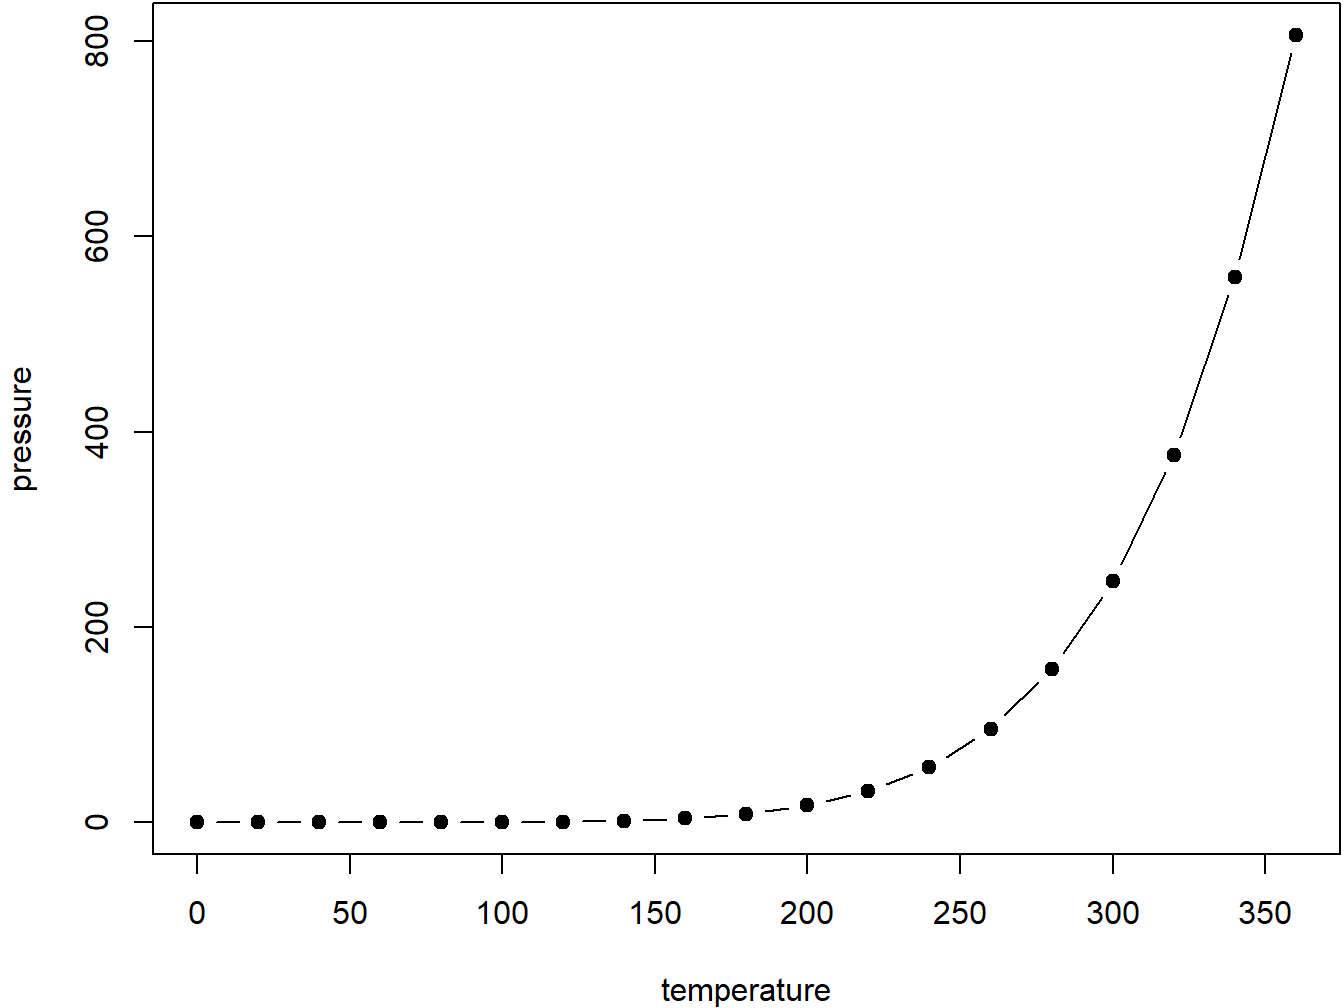
\includegraphics[width=0.8\linewidth]{Aplikasi-Komputer---Biostatistika_files/figure-latex/nice-fig-1} 

}

\caption{Here is a nice figure!}\label{fig:nice-fig}
\end{figure}

Reference a figure by its code chunk label with the \texttt{fig:} prefix, e.g., see Figure \ref{fig:nice-fig}. Similarly, you can reference tables generated from \texttt{knitr::kable()}, e.g., see Table \ref{tab:nice-tab}.

\begin{Shaded}
\begin{Highlighting}[]
\NormalTok{knitr}\SpecialCharTok{::}\FunctionTok{kable}\NormalTok{(}
  \FunctionTok{head}\NormalTok{(iris, }\DecValTok{20}\NormalTok{), }\AttributeTok{caption =} \StringTok{\textquotesingle{}Here is a nice table!\textquotesingle{}}\NormalTok{,}
  \AttributeTok{booktabs =} \ConstantTok{TRUE}
\NormalTok{)}
\end{Highlighting}
\end{Shaded}

\begin{table}

\caption{\label{tab:nice-tab}Here is a nice table!}
\centering
\begin{tabular}[t]{rrrrl}
\toprule
Sepal.Length & Sepal.Width & Petal.Length & Petal.Width & Species\\
\midrule
5.1 & 3.5 & 1.4 & 0.2 & setosa\\
4.9 & 3.0 & 1.4 & 0.2 & setosa\\
4.7 & 3.2 & 1.3 & 0.2 & setosa\\
4.6 & 3.1 & 1.5 & 0.2 & setosa\\
5.0 & 3.6 & 1.4 & 0.2 & setosa\\
\addlinespace
5.4 & 3.9 & 1.7 & 0.4 & setosa\\
4.6 & 3.4 & 1.4 & 0.3 & setosa\\
5.0 & 3.4 & 1.5 & 0.2 & setosa\\
4.4 & 2.9 & 1.4 & 0.2 & setosa\\
4.9 & 3.1 & 1.5 & 0.1 & setosa\\
\addlinespace
5.4 & 3.7 & 1.5 & 0.2 & setosa\\
4.8 & 3.4 & 1.6 & 0.2 & setosa\\
4.8 & 3.0 & 1.4 & 0.1 & setosa\\
4.3 & 3.0 & 1.1 & 0.1 & setosa\\
5.8 & 4.0 & 1.2 & 0.2 & setosa\\
\addlinespace
5.7 & 4.4 & 1.5 & 0.4 & setosa\\
5.4 & 3.9 & 1.3 & 0.4 & setosa\\
5.1 & 3.5 & 1.4 & 0.3 & setosa\\
5.7 & 3.8 & 1.7 & 0.3 & setosa\\
5.1 & 3.8 & 1.5 & 0.3 & setosa\\
\bottomrule
\end{tabular}
\end{table}

You can write citations, too. For example, we are using the \textbf{bookdown} package \citep{R-bookdown} in this sample book, which was built on top of R Markdown and \textbf{knitr} \citep{xie2015}. Kembali keatas \ref{a1-pengenalan}

  \bibliography{book.bib,packages.bib}

\end{document}
